% !TEX root = ../master.tex

\vspace*{.5cm}
\section{bibliothek am meer}
\begin{center}
\emph{Diana Wolf}
\end{center}
\vspace*{1cm}


%body
\hypertarget{zeigen-sie-uns-den-ort-in-ihrer-bibliothek-an-dem-sie-die-meiste-zeit-verbringen.-was-ist-das-fuxfcr-ein-ort-wieso-sind-sie-die-meiste-zeit-dort}{%
\subsubsection*{Zeigen Sie uns den Ort in Ihrer Bibliothek, an dem Sie die
meiste Zeit verbringen. Was ist das für ein Ort? Wieso sind Sie die
meiste Zeit
dort?}\label{zeigen-sie-uns-den-ort-in-ihrer-bibliothek-an-dem-sie-die-meiste-zeit-verbringen.-was-ist-das-fuxfcr-ein-ort-wieso-sind-sie-die-meiste-zeit-dort}}

\begin{center}
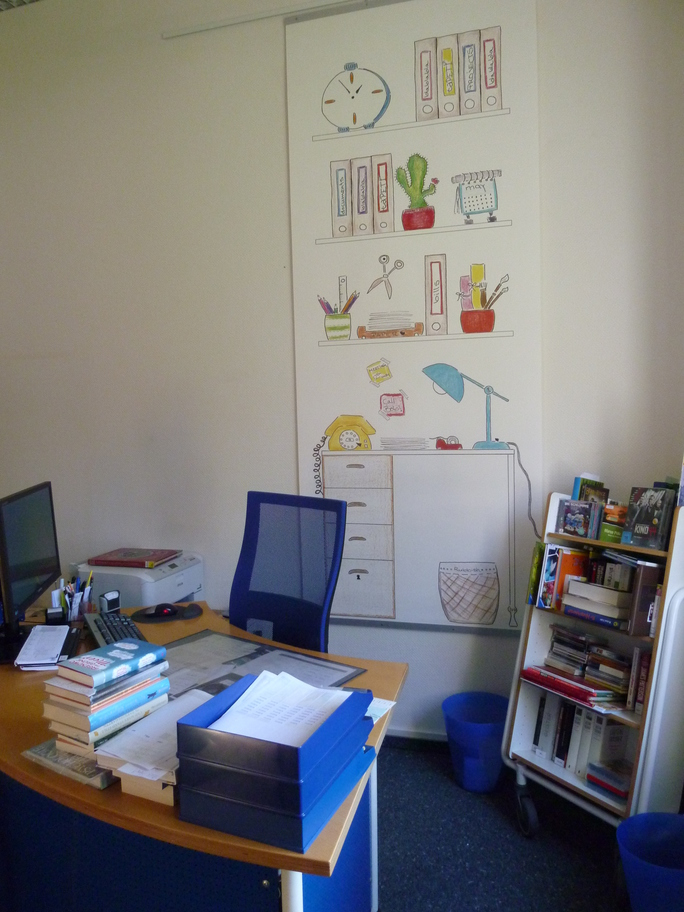
\includegraphics{am-meer/img/auskunft.jpg}
\end{center}

Es ist eigentlich der Auskunftsplatz, aber hier laufen alle Fäden
zusammen und man hat aus dem Hintergrund heraus einen guten Überblick
über den Bibliotheksbetrieb. Ganz nach dem Motto: Sehen und gesehen
werden.

\hypertarget{was-wuxfcrden-sie-vermissen-wenn-es-nicht-mehr-da-wuxe4re-wieso-wuxfcrden-sie-es-vermissen}{%
\subsubsection*{Was würden Sie vermissen, wenn es nicht mehr da wäre? Wieso
würden Sie es
vermissen?}\label{was-wuxfcrden-sie-vermissen-wenn-es-nicht-mehr-da-wuxe4re-wieso-wuxfcrden-sie-es-vermissen}}

\begin{center}
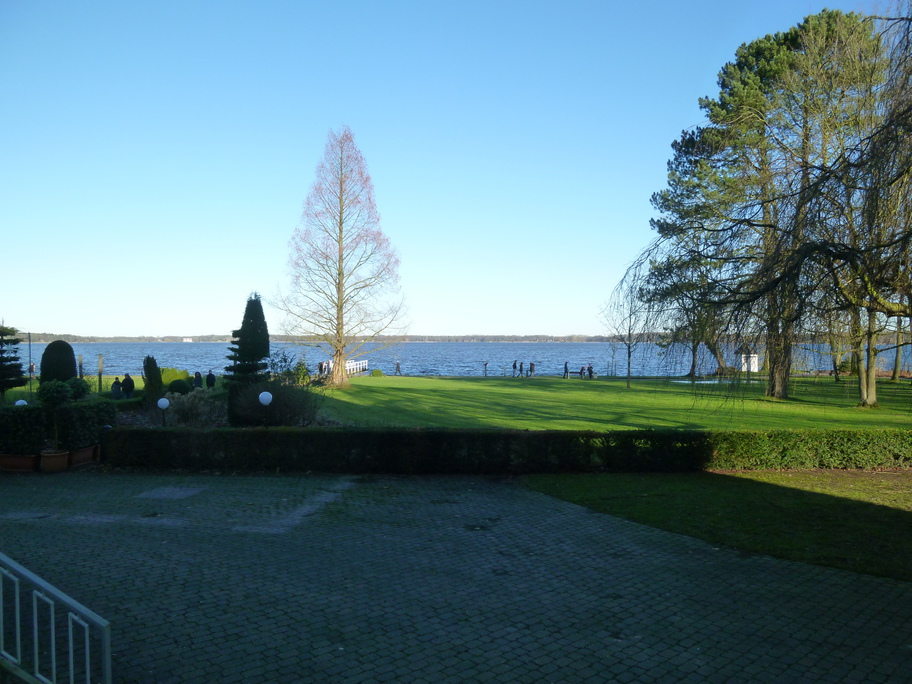
\includegraphics[width=0.5\textwidth]{am-meer/img/ausblick.jpg}
\end{center}

Die Lage am Zwischenahner Meer war ein Grund für den Bibliotheksnamen
\enquote{bibliothek am meer} und ohne diese Aussicht wäre die
Aufenthaltsqualität nur halb so gut.

\hypertarget{was-stuxf6rt-sie-an-ihrer-bibliothek-beziehungsweise-was-wuxfcrden-sie-gerne-verbessern-wieso-stuxf6rt-sie-das-jetzt-noch}{%
\subsubsection*{Was stört Sie an Ihrer Bibliothek beziehungsweise was würden
Sie gerne verbessern? Wieso stört Sie das jetzt
(noch)?}\label{was-stuxf6rt-sie-an-ihrer-bibliothek-beziehungsweise-was-wuxfcrden-sie-gerne-verbessern-wieso-stuxf6rt-sie-das-jetzt-noch}}

\begin{center}
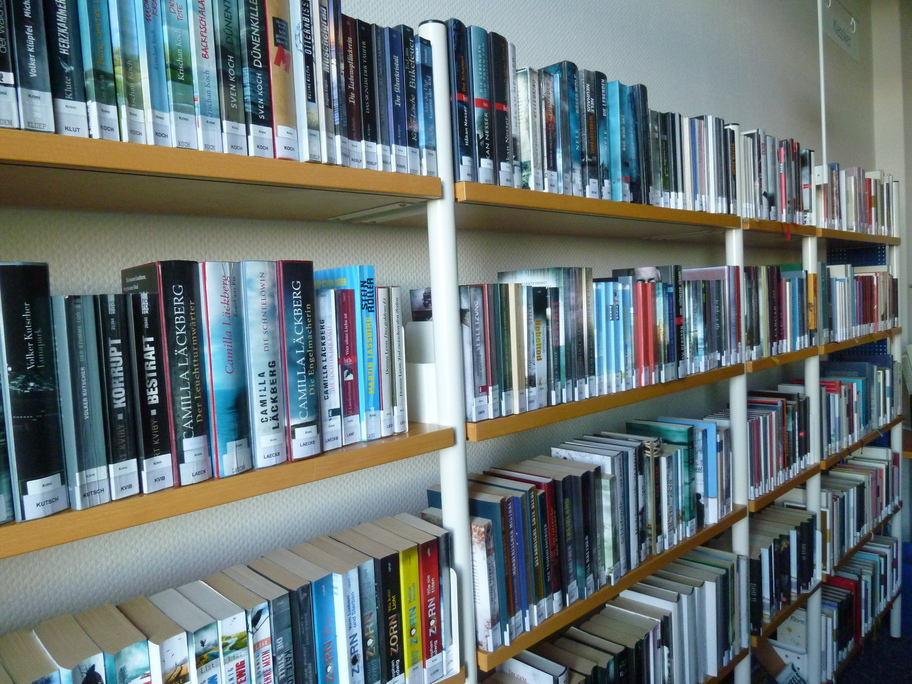
\includegraphics[width=0.5\textwidth]{am-meer/img/platzmangel.jpg}
\end{center}

Ein chronischer Platzmangel herrscht wohl in jeder Bibliothek. Der
tägliche Spagat zwischen maximalem Angebot und ansprechender
Präsentation der Titel gelingt nicht immer.

\hypertarget{zeigen-sie-uns-spuren-der-bibliotheksnutzung.-gibt-es-dazu-eine-geschichte}{%
\subsubsection*{Zeigen Sie uns Spuren der Bibliotheksnutzung. Gibt es dazu eine
Geschichte?}\label{zeigen-sie-uns-spuren-der-bibliotheksnutzung.-gibt-es-dazu-eine-geschichte}}

\begin{center}
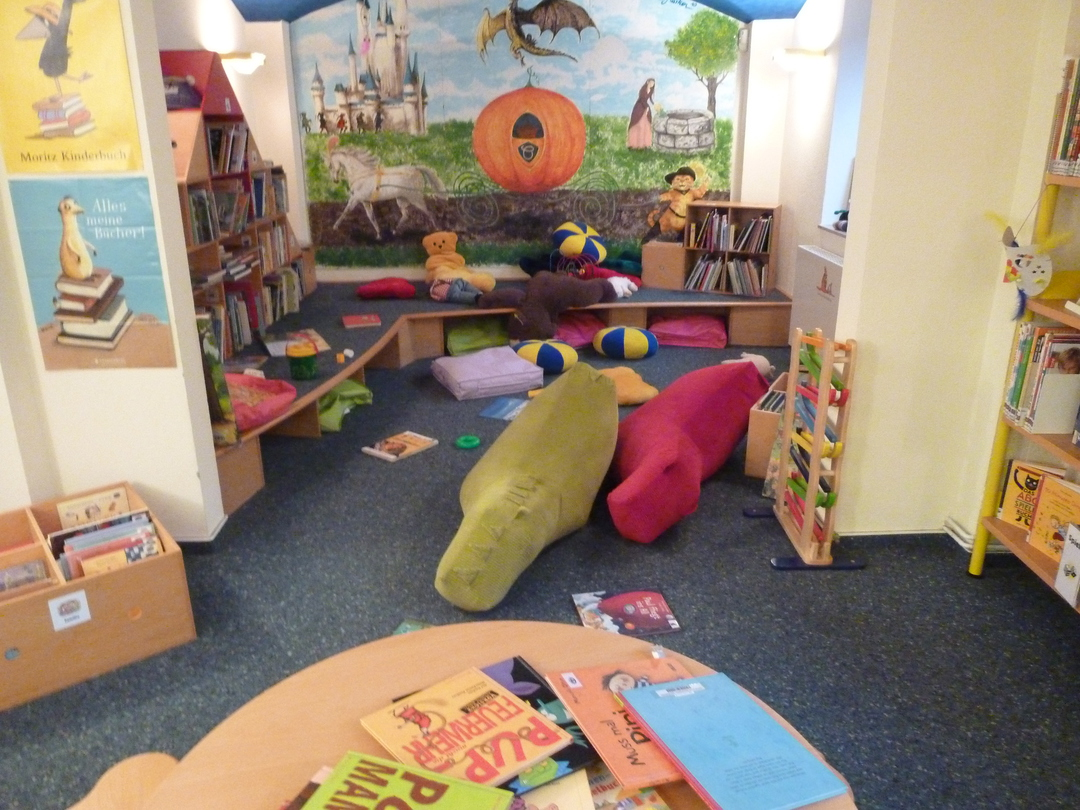
\includegraphics{am-meer/img/bilderbuchecke.jpg}
\end{center}

Das Ergebnis eines ganz normalen Samstagvormittags. Immer wieder schön,
wenn die Bilderbuchecke in der Kinderbibliothek auch ordentlich bespielt
wird.

\hypertarget{was-haben-sie-was-die-anderen-nicht-haben-warum-haben-sie-das-sollten-andere-es-auch-in-ihren-bibliotheken-haben}{%
\subsubsection*{Was haben Sie, was die anderen nicht haben? Warum haben Sie
das? Sollten andere es auch in ihren Bibliotheken
haben?}\label{was-haben-sie-was-die-anderen-nicht-haben-warum-haben-sie-das-sollten-andere-es-auch-in-ihren-bibliotheken-haben}}

\begin{center}
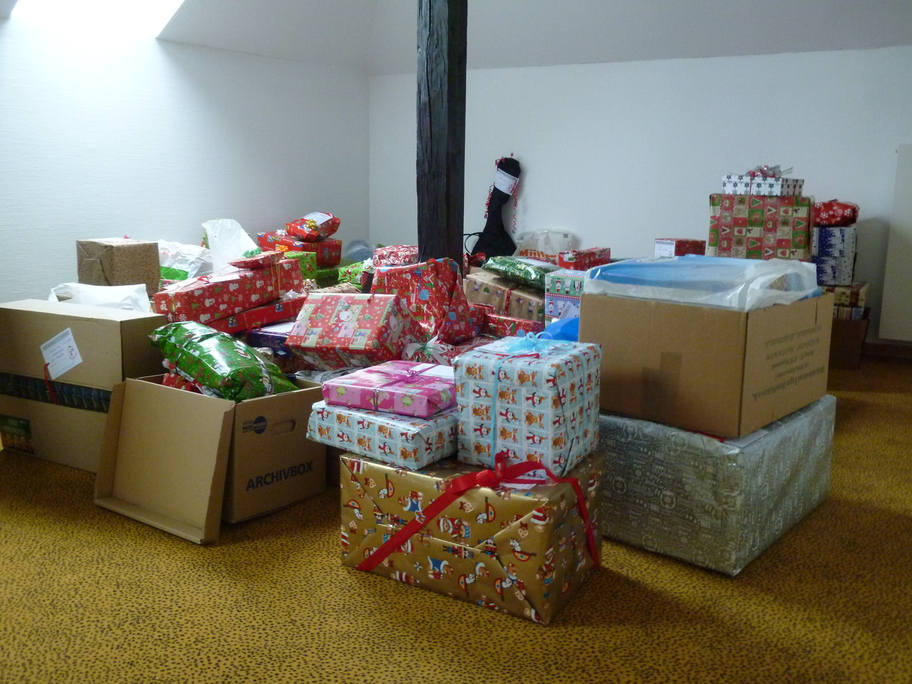
\includegraphics{am-meer/img/projekt-wunschbaum.jpg}
\end{center}

Mitte Dezember darf sich das Team der Bibliothek immer ein wenig wie der
Weihnachtsmann fühlen. Wir unterstützen aktiv das Projekt
\enquote{Wunschbaum} des Vereins \enquote{Glücksbringer am Meer}.
Vielleicht auch eine Form sozialer Bibliotheksarbeit.

\hypertarget{ihre-bibliothek-name-adresse-spezialisierung-was-man-noch-uxfcber-sie-wissen-sollte}{%
\subsubsection*{Ihre Bibliothek (Name, Adresse, Spezialisierung, was man noch
über sie wissen
sollte)?}\label{ihre-bibliothek-name-adresse-spezialisierung-was-man-noch-uxfcber-sie-wissen-sollte}}

\enquote{bibliothek am meer}, Auf dem Hohen Ufer 20, 26160 Bad
Zwischenahn, Bibliothek mit Qualität und Siegel der Büchereizentrale
Niedersachsen

%autor
\begin{center}\rule{0.5\linewidth}{\linethickness}\end{center}

\textbf{Diana Wolf}, Leiterin der Bibliothek